\section{Additional Experimental Results}

% ###################################
\begin{table}[t]
    \centering
    \caption{\textbf{Ablations on pixel-space generation.} 
    We study generation directly in pixel space (without VAE). Applying the same MAE recipe as in latent space yields higher FID, indicating that pixel-space generation is more challenging. Combining MAE with ConvNeXt-V2 helps close this gap. Latent-space results shown for reference. The results below follow the ablation setting (B/16 model for pixel-space, 100 epochs).
    }
    \label{tab:ablation_latent_vs_pixel}
    % \vspace{.5em}
    \tablestyle{6pt}{1.05}
    \tablefontsize
    \begin{tabular}{l r r}
    \toprule
    & \multicolumn{2}{c}{FID (100-epoch)} \\
    \cmidrule{2-3}
    feature encoder $\phi$ & latent (B/2) & pixel (B/16) \\
    \midrule
    MAE (width 256, epoch 192) & \cg 8.46 & 32.11 \\
    MAE (width 640, epoch 1280) + cls ft. & \cg 3.36 & 9.35 \\
    ~+ MAE w/ ConvNeXt-V2 & \cg - & \textbf{3.70} \\
    \bottomrule
    \end{tabular}
\end{table}
% ###################################

% ###################################
\begin{table}[t]
    \centering
    \caption{\textbf{Pixel-space generation: from ablation to final setting.} Beyond the ablation setting, we compare the settings that lead to the results in Table~\ref{tab:in256_pixel}.
    }
    % \vspace{.5em}
\label{tab:ablation_final_pixel}
    \tablestyle{6pt}{1.05}
    \tablefontsize
    \begin{tabular}{l |l r| c}
    \toprule
    case & arch & ep & FID \\
    \midrule
    (a) baseline (from Table~\ref{tab:ablation_latent_vs_pixel}) & B/16 & 100 & 3.70 \\
    \midrule
    (b) longer + hyper-param. & B/16 & 320 & 2.19 \\
    (c) longer & B/16 & 640 & 1.76 \\
    (d) larger model & L/16  & 640 & \textbf{1.61} \\
    \bottomrule
    \end{tabular}
\end{table}
% ###################################


% Allow floats to take up more of a page
\renewcommand{\topfraction}{0.95}
\renewcommand{\bottomfraction}{0.95}
\renewcommand{\textfraction}{0.05}
\renewcommand{\floatpagefraction}{0.9}

% ======================================
\begin{table}[t]
    \centering
    \caption{\textbf{Ablation on kernel normalization.}
    Softmax normalization over both the $\x$ and $\y$ axes performs better. On the other hand, even using no normalization performs decently, showing the robustness of our method.
    (Setting: B/2 model, 100 epochs)
    }
    \label{tab:kernel_normalization}
    % \vspace{.5em}
    \tablestyle{6pt}{1.0}
    \tablefontsize
    \begin{tabular}{l r}
    \toprule
    kernel normalization & FID \\
    \midrule
    softmax over $\x$ and $\y$ (default) & \textbf{8.46} \\
    softmax over $\y$ & 8.92 \\
    no normalization & 10.54 \\
    \bottomrule
    \end{tabular}
    \vspace{-.5em}
\end{table}
% ======================================

\subsection{Ablations on Pixel-Space Generation}
\label{section:exp_pixel_space}

We provide more ablations on pixel-space generation in Table~\ref{tab:ablation_latent_vs_pixel} and \ref{tab:ablation_final_pixel}.
Table~\ref{tab:ablation_latent_vs_pixel} compares the effect of the feature encoder on the pixel-space generator. 
It shows that the choice of feature encoder plays a more significant role in pixel-space generation quality.
A weaker MAE encoder yields an FID of 32.11, whereas a stronger MAE encoder improves performance to an FID of 9.35.
We further add another feature encoder, ConvNeXt-V2 \cite{woo2023convnext}, which is also pre-trained with the MAE objective. This further improves the result to an FID of 3.70.

Table~\ref{tab:ablation_final_pixel} reports the results of training longer and using a larger model. Due to limited time, we train pixel-space models for 640 epochs (\vs~the latent counterpart's 1280); we expect that longer training would yield further improvements.
We achieve an FID of 1.61 for pixel-space generation. This is our result in the main paper (Table~\ref{tab:in256_pixel}).

% ###################################
\begin{figure}[t]
    \centering
    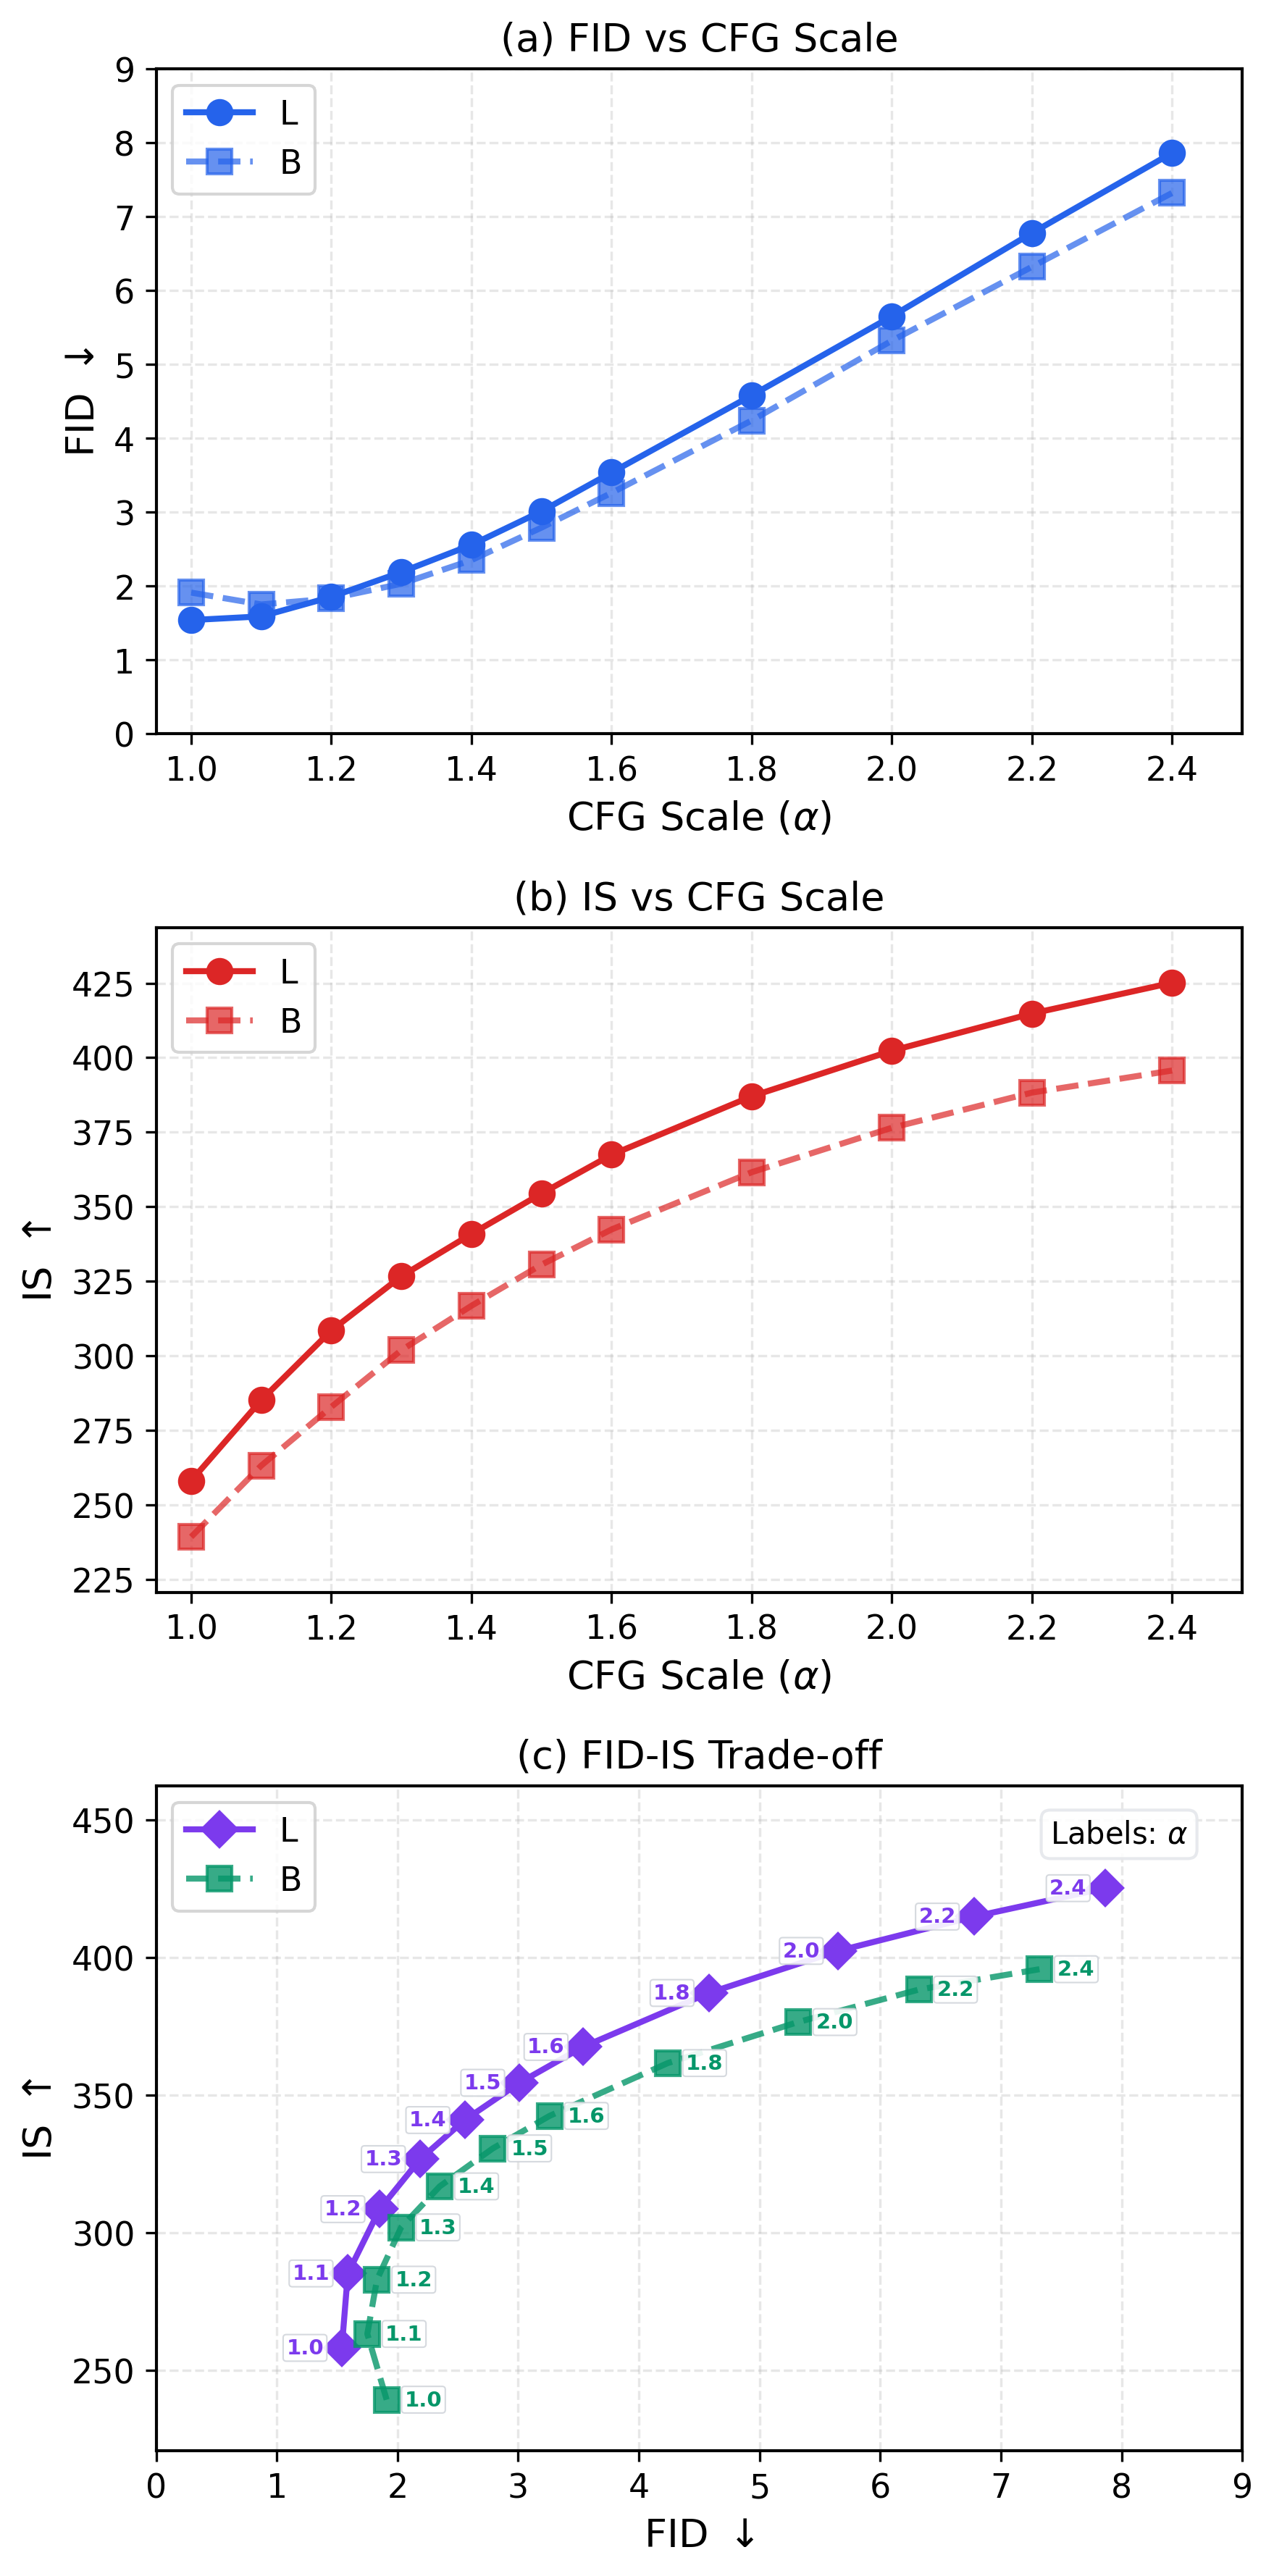
\includegraphics[width=0.65\linewidth]{figures/cfg_tradeoff_combined.png}
    \vspace{-.75em}
    \caption{\textbf{Effect of CFG scale $\alpha$.} 
    \textbf{(a)}: FID vs.~$\alpha$.
    \textbf{(b)}: IS vs.~$\alpha$.
    \textbf{(c)}: IS vs.~FID.
    We show the L/2 (solid) and B/2 (dashed) models.
    Consistent with common observations in diffusion-/flow-based models, the CFG scale effectively trades off distributional coverage (as reflected by FID) against per-image quality (measured by IS).
    Notably, with the L/2 model, the optimal FID is achieved at $\alpha{=}1.0$, which is often regarded as ``w/o CFG'' in diffusion-/flow-based models. For B/2, the optimal FID is achieved at $\alpha{=}1.1$.
    }
    \label{fig:cfg_tradeoff}
    \vspace{-1.5em}
\end{figure}
% ###################################


\subsection{Ablation on Kernel Normalization}
\label{sec:appendix_kernel_normalizatio}

In Eq.~(\ref{eq:VZZ}), our drifting field is weighted by normalized kernels, which can be written as:
\begin{equation}
\V(\x) = \mathbb E_{p,q} [\tilde{k}(\x, \yp) \tilde{k}(\x, \yn) (\yp - \yn)],
\end{equation}
where $\tilde{k}(\cdot, \cdot)=\frac{1}{Z}k(\cdot, \cdot)$ denotes the normalized kernel.
In principle, this normalization is approximated by a softmax operation over the axis of $\y$ samples. Our implementation (Alg.~\ref{alg:drift_code}) further applies softmax over the axis of $\x$ samples. We compare these designs, along with another variant without normalization ($Z=1$).

Table~\ref{tab:kernel_normalization} compares the three designs. Using the $\y$-only softmax performs well (8.92 FID), whereas using both $\x$ and $\y$ softmax improves the result (8.46 FID). On the other hand, even without normalization, performance remains decent, demonstrating the robustness of our method.

We note that all three variants satisfy the equilibrium condition $\V_{p,q}(\x) = \mathbf{0}$ when $p=q$. This explains why all variants perform reasonably well and why even the destructive setting (no normalization) avoids catastrophic failure.

\subsection{Ablation on CFG}
\label{section:exp_cfg}

In \cref{fig:cfg_tradeoff}, we investigate the CFG scale $\alpha$ used at inference time.
It shows that the CFG formulation developed for our models exhibits behavior similar to that observed in diffusion-/flow-based models.
Increasing the CFG scale leads to higher IS values, whereas beyond the FID sweet spot, further increases in IS come at the cost of worse FID.

Notably, with our best model (L/2), the optimal FID is achieved at $\alpha{=}1.0$, which is often regarded as ``w/o CFG'' in diffusion-/flow-based models (even though their ``w/o CFG'' setting can reduce NFE by half). 
While our method need not run an unconditional model at inference time (in contrast to standard CFG), training is influenced by the use of unconditional real samples as negatives.

% ###################################
\begin{figure}[t]
    \centering
    % Header row
    \begin{minipage}{0.49\linewidth}
        \centering
        \makebox[0.28\linewidth]{\hspace{1pt}\scriptsize \textbf{\textcolor{orange}{Generated}}}%
        \makebox[0.72\linewidth]{\scriptsize \textbf{\textcolor{blue}{Retrieved}}}
    \end{minipage}
    \hfill
    \begin{minipage}{0.49\linewidth}
        \centering
        \makebox[0.28\linewidth]{\hspace{5pt}\scriptsize \textbf{\textcolor{orange}{Generated}}}%
        \makebox[0.72\linewidth]{\hspace{5pt}\scriptsize \textbf{\textcolor{blue}{Retrieved}}}
    \end{minipage}
    \vspace{1pt}

    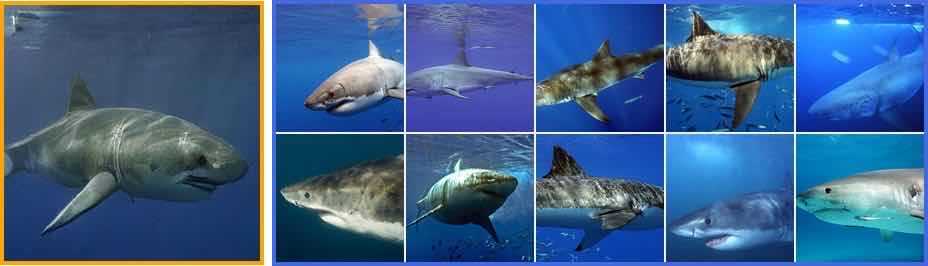
\includegraphics[width=0.49\linewidth]{figures/samples/nn_new/nn_vis_0004_class002_sim0.945.jpg}\hfill
    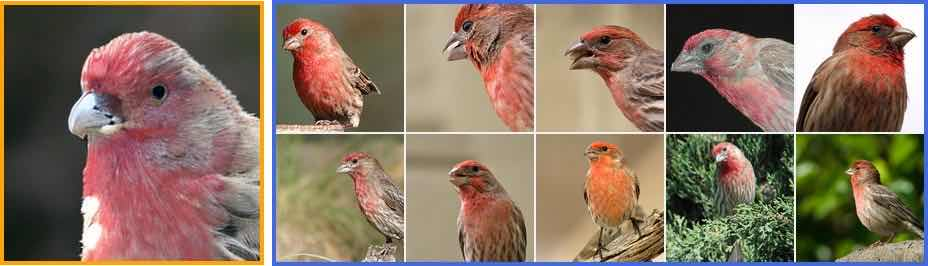
\includegraphics[width=0.49\linewidth]{figures/samples/nn_new/nn_vis_0025_class012_sim0.918.jpg}\\[1pt]
    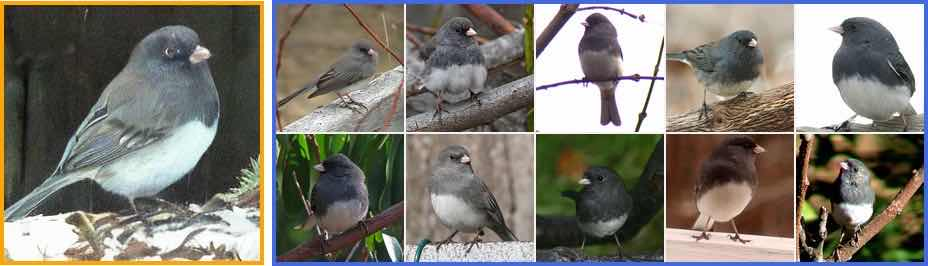
\includegraphics[width=0.49\linewidth]{figures/samples/nn_new/nn_vis_0027_class013_sim0.902.jpg}\hfill
    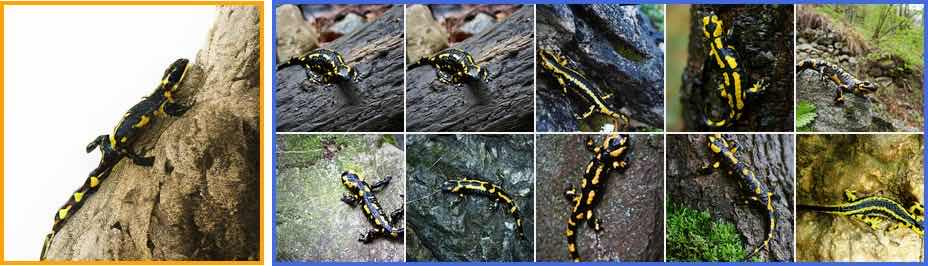
\includegraphics[width=0.49\linewidth]{figures/samples/nn_new/nn_vis_0050_class025_sim0.899.jpg}\\[1pt]
    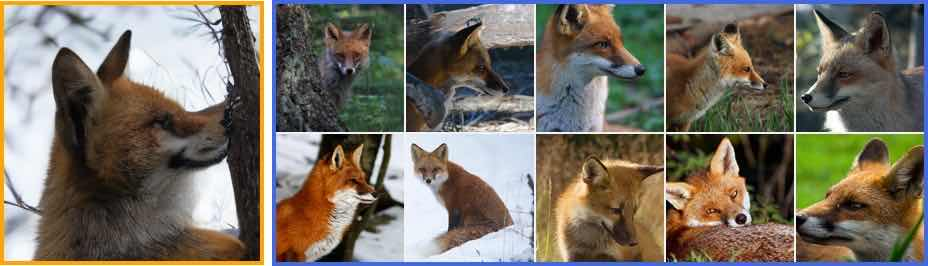
\includegraphics[width=0.49\linewidth]{figures/samples/nn_new/nn_vis_0554_class277_sim0.919.jpg}\hfill
    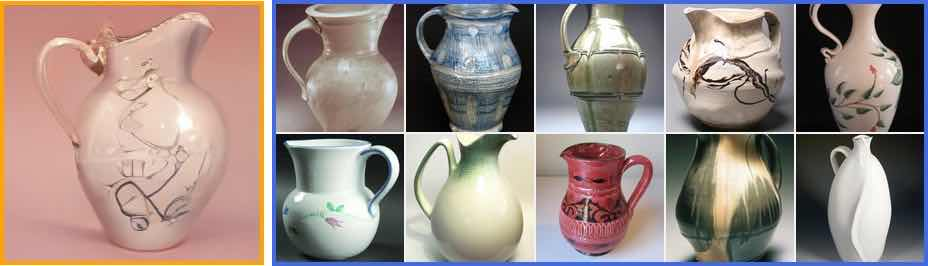
\includegraphics[width=0.49\linewidth]{figures/samples/nn_new/nn_vis_1451_class725_sim0.866.jpg}\\[1pt]
    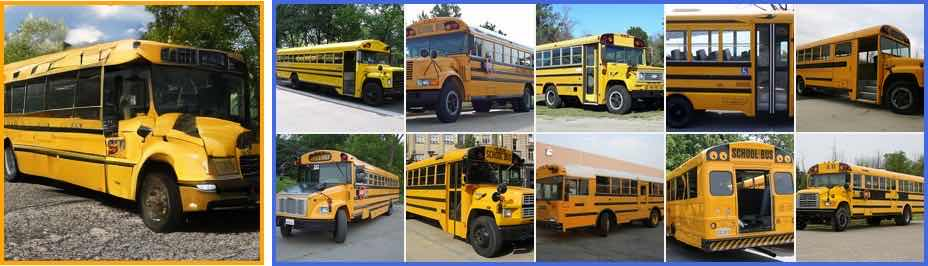
\includegraphics[width=0.49\linewidth]{figures/samples/nn_new/nn_vis_1559_class779_sim0.936.jpg}\hfill
    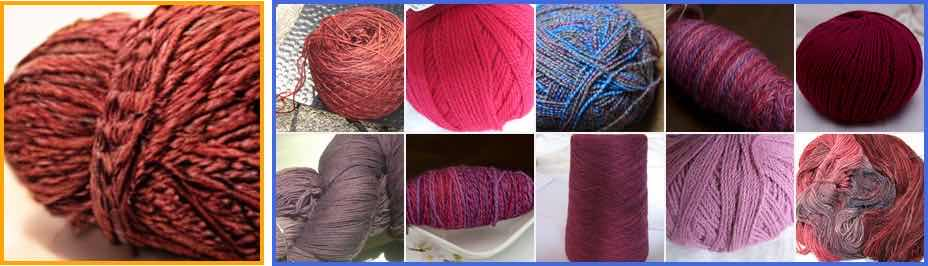
\includegraphics[width=0.49\linewidth]{figures/samples/nn_new/nn_vis_1822_class911_sim0.915.jpg}\\[1pt]
    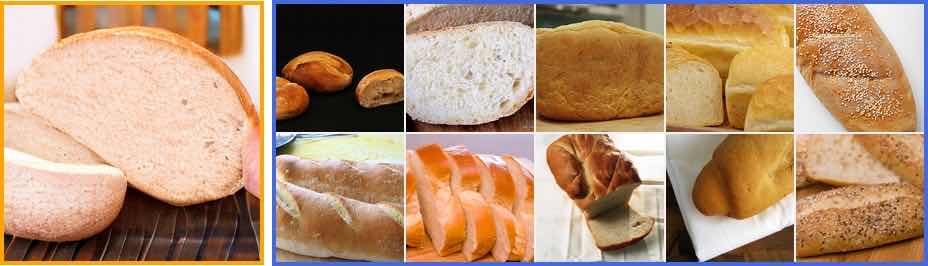
\includegraphics[width=0.49\linewidth]{figures/samples/nn_new/nn_vis_1861_class930_sim0.862.jpg}\hfill
    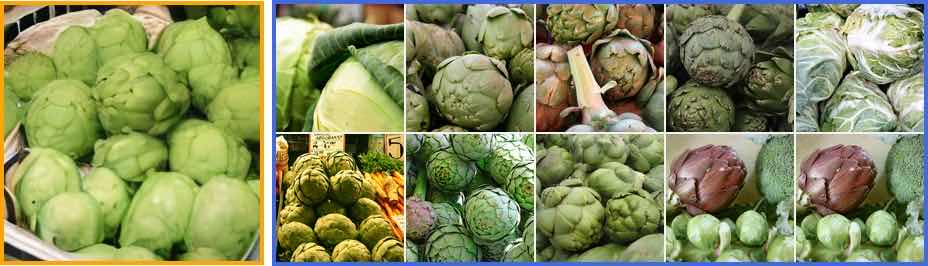
\includegraphics[width=0.49\linewidth]{figures/samples/nn_new/nn_vis_1889_class944_sim0.895.jpg}\\[1pt]
    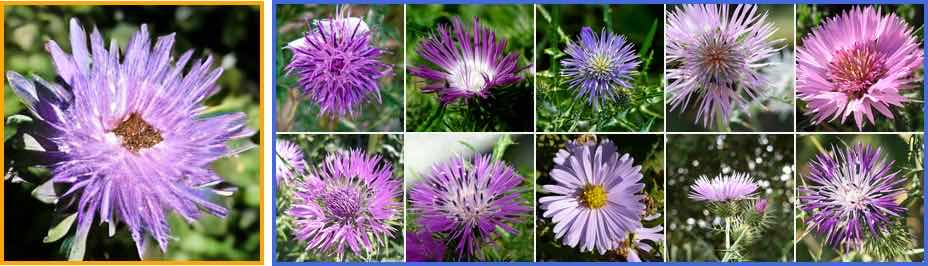
\includegraphics[width=0.49\linewidth]{figures/samples/nn_new/nn_vis_1893_class946_sim0.906.jpg}\hfill
    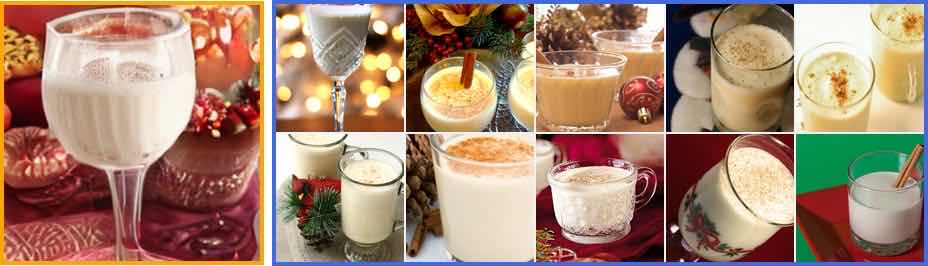
\includegraphics[width=0.49\linewidth]{figures/samples/nn_new/nn_vis_1938_class969_sim0.896.jpg}
    \caption{\textbf{Nearest neighbor analysis.} Each panel shows a \textcolor{orange}{{generated sample}} together with its top-10 nearest \textcolor{blue}{real images}. The nearest neighbors are retrieved from the ImageNet training set based on the cosine similarity using a CLIP encoder \cite{radford2021learning}. 
    Our method generates novel images that are visually distinct from their nearest neighbors.}
    \label{fig:nearest_neighbors}
    \vspace{-1.5em}
\end{figure}
% ###################################

\subsection{Nearest Neighbor Analysis}

In \cref{fig:nearest_neighbors}, we show generated images together with their nearest real images. The nearest neighbors are retrieved from the ImageNet training set using CLIP features. 
These visualizations suggest that our method generates novel images that are visually distinct from their nearest neighbors, rather than merely memorizing training samples.

\subsection{Qualitative Results}
\label{sec:appendix_qualitative_results}

Fig.~\ref{fig:latent_uncurated_samples_1}-\ref{fig:latent_uncurated_samples_4} show uncurated samples from our model.
Fig.~\ref{fig:comparison_imf_1}-\ref{fig:comparison_imf_5} provide side-by-side comparison with improved MeanFlow (iMF) \cite{geng2025improved}, the current state-of-the-art one-step method.